Una vez fijados los objetivos a abordar, en este capítulo se va a
describir la infraestructura concreta en la que nos hemos apoyado
para desarrollar las soluciones, tanto hardware como software.

\section{3DR Solo Dron}
Para este Trabajo Fin de Grado se ha elegido el dron 3DR\cite{3dr} Solo distribuido por la empresa norteamericana \footnote{\url{https://3dr.com/}}. Este dron se encuentra en una gama alta debido a sus capacidades \footnote{\url{https://3dr.com/solo-drone/specs/}}, tales como batería, distancia de comunicacion y potencia, cualidades que lo hacen un dron muy versatil. Durante el desarrollo se ha usado la versión oficial del firmware de 3DR 2.4.2. Se eligió esa debido a que era una versión estable. A bordo de este dron se encuentra una placa estabilizadora Pixhawk 2.

\begin{figure}[H]
  \centering
  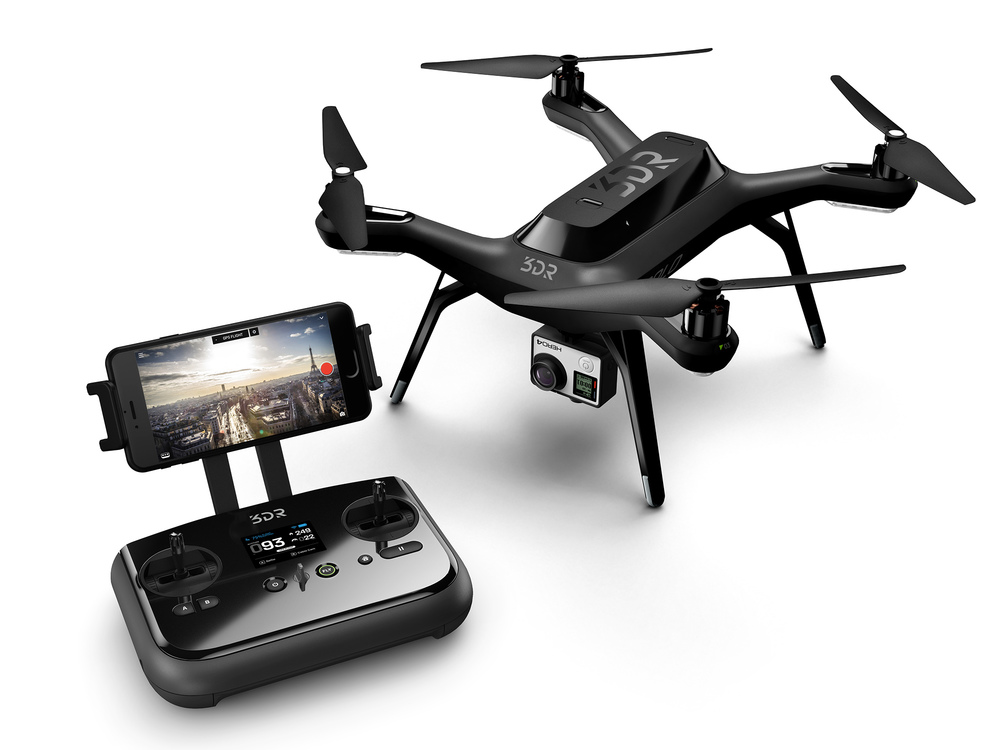
\includegraphics[scale=1]{imagenes/3drSoloDron.jpg}
  \caption{3DR Solo Drone}
  \label{fig:3drsolodrone}
\end{figure}

La CPU que tiene este dron es la ArduIMU,\footnote{\url{https://3dr.com/support/articles/arduimu_v3_kit/}}, es una tarjeta de Unidad de Medida Inercial (IMU) que integra un procesador compatible con Arduino y que capaz de ejecutar Attitude Heading Reference System (AHRS), basado en el algoritmo DCM (Direct Cosine Matrix) de Bill Premerlani.

La tarjeta IMU consta de un acelerómetro de 3 ejes y tres sensores giroscópicos, un regulador de tensión dual (3.3V y 5V), un puerto de GPS, un Atmega328 @ 16MHz (como el Arduino Duemilanova) y 3 LEDs de estado.

Es importante aclarar que la ArduIMU de la figura \ref{fig:arduimu} no es ninguna placa de navegación o piloto automático, sólo una placa de orientación y se puede utilizar en cualquier cosa en la que deseemos conocer su orientación con respecto al suelo – barcos, coches, aviones,
Cuenta con una MPU-6000 que integra un giroscopio y acelerómetro de 3 ejes y se comunica mediante el bus SPI, un magnetómetro HMC-5883L conectado mediante I2C y un Arduino Atmega328 de 16Mhz.

\begin{figure}[H]
  \centering
  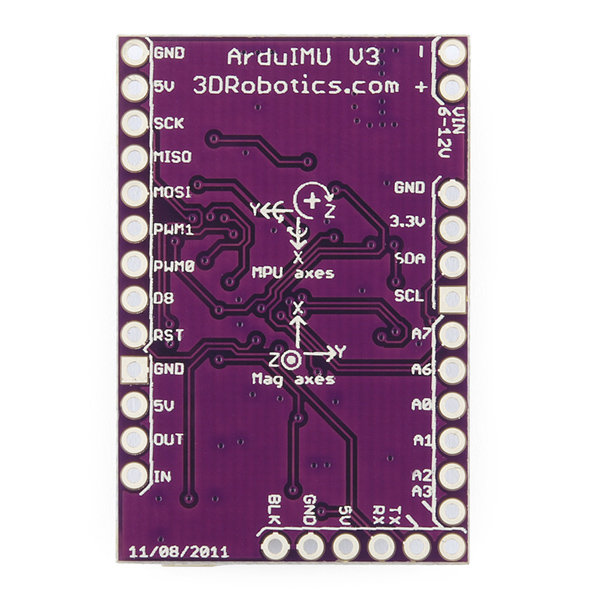
\includegraphics[scale=1]{imagenes/arduimutrasera.jpg}
  \caption{ArduIMU}
  \label{fig:arduimu}
\end{figure}

El mando proporciona los mecanismos de control y muestra los datos del vuelo en una pantalla a todo
color. Mediante el uso de antenas dobles de largo alcance, el mando actúa como el eje central para todas la
comunicaciones de la red Link 3DR via radio, recibe todas las comunicaciones de Solo y la aplicación, reenvía las salidas telemétricas a la aplicación y administra la transmisión de todas las entradas de control a Solo.

Este dron incluye una placa estabilizadora Pixhawk, esta placa es un desarrollo específico creado entre la "Pixhawk\cite{pixhawk} open hardware community" en colaboración con 3D Robotics y que vio como primer destinatario el 3DR Solo. Ofrece un interfaz que se apoya en el protocolo MAVLink que se describe en la sección \ref{fig:protocoloMavlink}. A través de estos comandos se le puede también enviar órdenes al piloto automático. El único modo de conectar con el 3DR Solo será a través del mando, debido a que únicamente él es capaz de levantar la red wifi a la que poder conectarse. En posteriores evoluciones de la versión que controlan tanto el dron como el mando, desde los foros oficiales de 3DR \footnote{\url{https://3drpilots.com/threads/connecting-directly-to-the-pixhawk-2-on-a-solo.7926/}}, comentan que ya se aborda la solución de que sea el propio dron quien levante la red wifi a la cual poder conectar y no tener que depender del enlace del mando.

\section{Protocolo MAVLink}
\label{sec:mavlink}

MAVLink\cite{mavlink} (Micro Air Vehicle Link) es un protocolo desarrollado para comunicar las placas estabilizadoras dotadas de piloto automático a los GCS (Ground Control Station) o estación de tierra con las aplicaciones desde las que se envía misiones y se monitoriza el cumplimiento de las mismas desde tierra.
MAVLink se publicó \footnote{\url{https://github.com/mavlink/mavlink/commit/a087528b8146ddad17e9f39c1dd0c1353e5991d5}} en 2009 por Lorenz Meier, con licencia LGPL. Aspira a convertirse en el protocolo standard en robótica aérea y se ha probado su funcionamiento en PX4, PIXHAWK, APM\footnote{Ardupilot Mega} y Parrot AR.Drone.

La lista completa de los comandos de este protocolo se encuentra en la pagina oficial de Mavlink\footnote{\url{http://mavlink.org/messages/common}}. La versión actual que se está utilizando en este TFG es la 2.0. 

Cada comando tiene un identificador único  el cual permite al dron reconocer la acción que se debe realizar. En función de este identificador los parámetros que se introducen a continuación dan la información necesaria al dron para actuar. Un ejemplo de la estructura del mensaje que se usa para GPS es el siguiente:
\begin{lstlisting}[frame=single]
type GpsStatus struct {
    SatellitesVisible  uint8      
    SatellitePrn       [20]uint8  
    SatelliteUsed      [20]uint8  
    SatelliteElevation [20]uint8  
    SatelliteAzimuth   [20]uint8  
    SatelliteSnr       [20]uint8  
}
\end{lstlisting}
Este mensaje trae la información del enlace actual con el GPS y se envía periódicamente en ciclos que se configura en los parámetros de conexión con el dispositivo.

Un ejemplo de los mensajes más importantes del protocolo y en el que se centra este TFG es el comando de velocidad. Este comando hace uso de la estructura del mensaje "SET\_POSITION\_TARGET\_LOCAL\_NED", en el cual se indican las velocidades lineales que debe seguir en cada eje (en m/s). Este comando, junto con el de ordenar la rotación, cuya estructura es la del mensaje "COMMAND\_LONG", permite tener control total sobre las velocidade del dron. 

En la figura \ref{fig:comunicacionMAVLink} se puede comprobar la de comunicación entre la estación de tierra y cada componente se establece una conexión, en la cual continuamente se intercambian mensajes con información, ya sea para comunicar una acción, reclamar el estado de algún componente interno, como podría ser la batería, o un simple ACK para mantener la conexión activa.


\begin{figure}[H]
  \centering
  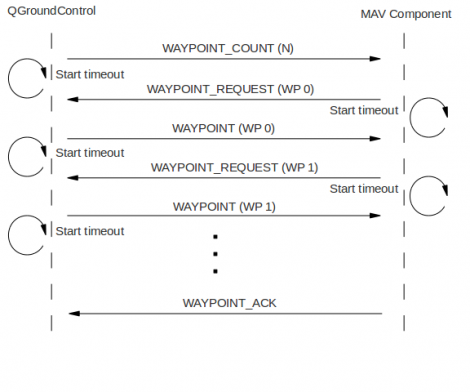
\includegraphics[scale=0.5]{imagenes/comunicacionMavLink.png}
  \caption{Comunicación MAVLink}
  \label{fig:comunicacionMAVLink}
\end{figure}

\subsection{MavProxy}
\label{sec:MavProxy}

MavProxy es un módulo controlador multihilo que simplifica el uso del protocolo MAVLink desde aplicaciones en python. Es un GCS totalmente funcional (sistema de comunicación grupal) para UAV, versión
1.4.38 es el utilizado en este trabajo fin de grado . Es un GCS minimalista, portátil y extensible para
cualquier UAV que soporte el protocolo MAVLink. Tiene una serie de características clave, que incluyen
la capacidad de reenviar mensajes de UAV a través de la red a través de UDP (User Datagram
Protocol) a otros programas de estación terrestre en otros dispositivos.

Tiene como principales caracteristicas:

\begin{itemize}
\item Es una aplicación de línea de comandos y consola. Hay complementos incluidos en MAVProxy
para proporcionar una GUI básica.
\item Está escrito en Python.
\item Es de código abierto.
\item Es portátil; debería ejecutarse en cualquier sistema operativo POSIX con python, pyserial y función
llamadas, lo que significa Linux, OS X, Windows y otros.
\item Admite módulos cargables, y tiene módulos para admitir consolas, mapas en movimiento,
joysticks, seguidores de antena, etc.
\end{itemize}

El flujo de la información y la operación del controlador sigue el siguiente funcionamiento:

\begin{itemize}
\item El controlador comienza a ejecutar todos los hilos diferentes, abriendo su comunicación canales y definiendo la información que estaría en cada uno. Hace uso de dos canales de comunicación basados en Pose3D, uno para publicar la posición del vehículo y actitud y otra para recibir órdenes de puntos de referencia; y un CMDVel canal para los comandos de aterrizaje.
\item Los mensajes de MAVLink entran en el controlador y se interpretan para obtener la información de posición y actitud del vehículo. Adquirida esta  información se trata para transformarla en estándares JdeRobot (Pose3D). Latitud y la longitud se transforman en coordenadas xyz globales, utilizando WGS84 como la Tierra modelo, y la actitud de ángulos de Euler se transforman en cuaterniones.
\item Pose3D está escrito en las clases locales correspondientes de forma controlada, haciendo uso de lock (librería que nos permite excluir ciertas variables para su uso).
\item Las clases se publican en los canales de ICE correspondientes a medida que se ejecutan los hilos, para permitir que otras aplicaciones de JdeRobot puedan acceder a ellos.
\item Los comandos de aterrizaje se reciben a través de Extra y comandos de velocidad a través de CmdVel. La información se extrae de las clases correspondientes.
\item Los comandos se traducen a mensajes MAVLink y se envían a la placa Pixhawk.
\end{itemize}

Se puede ver que cada subproceso tiene una tarea pero no tienen la misma carga de trabajo.
Por esta razón, el tiempo del ciclo de control de cada hilo es diferente. A pesar de la los hilos tienen diferentes ritmos, el módulo funciona con éxito en todas sus diferentes tareas.

MAVLink admite tipos de datos enteros de tamaño fijo, números de punto flotante de precisión simple IEEE 754, matrices de estos tipos de datos (por ejemplo, char [10]) y el campo especial de conversión de MAVLink, que se agrega automáticamente mediante el protocolo. Estos tipos están disponibles:

\begin{multicols}{3}
\begin{itemize}
\item char
\item uint8
\item int8
\item uint16
\item int16
\item uint32
\item int32
\item uint64
\item int64
\end{itemize}
\end{multicols}

Estos paquetes que se envían tienen la estructura de la imagen \ref{fig:protocoloMavlink}, y en la tabla \ref{tablaMAVLinkProtocolo} se hace referencia a cada uno de los campos con una breve explicación de cada uno de ellos:

\clearpage
\begin{figure}[H]
  \centering
  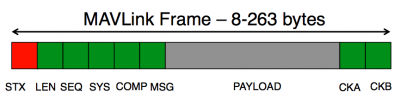
\includegraphics[scale=0.65]{imagenes/protocoloMavLink.png}
  \caption{Protocolo Mavlink}
  \label{fig:protocoloMavlink}
\end{figure}

\begin{center}
	\label{tablaMAVLinkProtocolo}
    \begin{tabular}{ | p{2cm} | p{2cm} | p{3cm} | p{5cm} |}
    \hline
    Índice del byte & Contenido & Valor & Explicación \\ \hline
    0 & Señal inicio paquete & 0xFE  & Indica el inicio de un nuevo paquete. \\ \hline
     1 & Longitud de la carga	& 0 - 255 & Indica la longitud de los datos que lleva. \\ \hline
     2 & Secuencia del paquete & 0 - 255 & Cada componente cuenta con su propia secuencia. Permite detectar paquetes perdidos. \\
    \hline
    3 & ID del sistema & 1 - 255 & ID del sistema emisor. Permite diferenciar MAVs en la misma red. \\
    \hline
    4 & ID del componente & 0 - 255	& ID del componente emisor. Permite diferenciar componentes en el mismo sistema, por ejemplo la IMU y la cámara.\\
    \hline
    5 & ID del mensaje	& 0 - 255 & Permite identificar los datos del paquete para su correcta decodificación.\\
    \hline
     6 to (n+6)  & Datos	& (0 - 255) bytes & Datos del mensaje, depende del ID del mensaje.\\
    \hline
   	(n+7) to (n+8) & Checksum &  & El checksum  incluye MAVLINK-CRC-EXTRA (protege el paquete de una decodificación errónea). \\ 
    \hline
    \end{tabular}
\end{center}



\section{JdeRobot}
\label{sec:jderobot}

JdeRobot\cite{jderobot} es un entorno desarrollado por el laboratorio de robótica de la Universidad Rey Juan Carlos, para el desarrollo de aplicaciones de robótica. Su última versión la 5.6 \footnote{\url{https://github.com/JdeRobot/JdeRobot}} se liberó el 9 de Octubre de 2017 y es la usada en este TFG. JdeRobot se compone de interfaces, drivers, utilidades y aplicaciones para el desarrollo de proyectos de robótica. Las aplicaciones y los drivers se comunican intercambiando mensajes entre sí utilizando interfaces ICE o interfaces ROS.
Algunos de los drivers más importantes que contiene:
\begin{enumerate}
\item Cameraserver. Para enviar imágenes y video a través del interfaz ICE camera.
\item Gazeboserver. Conjunto de plugins en el simulador Gazebo que ejercen de drivers entre las aplicaciones inteligentes y los robots simulados.
\item Ardrone\_server. Driver que conecta los sensores y actuadores del Parrot Ar-Drone a ICE \footnote{\url{http://jderobot.org/Amartinflorido-tfg}}. Esta escrito en C++, transforma el conjunto de comandos AT del drone en interfaces y viceversa, implementa los interfaces camera, cmdvel, navdata, extra y pose3D y permite acceder a la actitud del drone así como a sus 2 cámaras. Sirve también datos como el nivel de la batería y permite grabar vídeo o tomar fotos.
\end{enumerate}
Algunas de las herramientas disponibles en JdeRobot más usadas en este TFG son:
\begin{enumerate}
\item Cameraview. Una aplicación desarrollada en C++ capaz de recibir vídeo a través del interfaz camera.
\item UAV viewer. Aplicación desarrollada como control en tierra de robots aéreos. Permite teleoperar cualquier tipo de robot aéreo. Ofrece de forma visualmente atractiva datos como la actitud, velocidades lineales y angulares, ofrece también la posibilidad de visualizar videos servidos por el interfaz camera. \footnote{\url{http://jderobot.org/Amartinflorido-tfg}}.
\end{enumerate}

\subsection{Interfaces ICE relativos a los drones}
JdeRobot dispone de más de 30 interfaces pero en este cap\'itulo se explican los que se han utilizado durante este TFG:
\begin{itemize}
\item Pose3D. Utilizado para recoger los datos de actitud y la posici\'on de la aeronave.
\begin{lstlisting}[frame=single]
Pose3DData
  {
	float x;  /* x coord */
	float y;  /* y coord */
	float z;  /* z coord */
  	float h;  /* */
	float q0; /* qw */
	float q1; /* qx */
	float q2; /* qy */
	float q3; /* qz */
  };
\end{lstlisting}

\item CMDVel. Utilizado para enviar comandos de velocidad.
\begin{lstlisting}[frame=single]
	class CMDVelData
	{
		float linearX;
		float linearY;
		float linearZ;
		float angularX;
		float angularY;
		float angularZ;										
	};

\end{lstlisting}
\item Extra. Utilizado principalmente para las órdenes de despegue y aterrizaje.
\begin{lstlisting}[frame=single]

    void land() - land drone. 
    void takeoff() - takeoff drone. 
    void reset() 
    void recordOnUsb(bool record) 
    void ledAnimation(int type,float duration, float req) 
    void flightAnimation(int type, float duration) 
    void flatTrim() 
    void toggleCam() - switch camera. 
\end{lstlisting}

\end{itemize}

\section{Biblioteca de comunicaciones ICE}
\label{sec:ICE}
ICE\cite{ice} (Internet Communications Engine) es un \textit{middleware}  orientado a objetos que proporciona llamadas a procedimientos remotos, \textit{grid computing} y funcionalidad cliente / servidor desarrollada por ZeroC con una licencia GNU GPL y también una licencia privativa. Está disponible para C ++,
Java, .Net languages, Objective-C, Python, PHP y Ruby, en la mayoría de los sistemas operativos. También hay una versión para teléfonos móviles llamada Ice-e. 

ICE permite desarrollar aplicaciones distribuidas con un esfuerzo mínimo, abstraer al programador para que interactúe con una red de manera simple, usando interaces entre objetos distribuidos. El desarrollo de aplicaciones se enfoca así sólo en la lógica y no en las peculiaridades de la red. Es un \textit{middleware} multilenguaje, podemos implementar clientes y servidores en diferentes lenguajes de programación y en diferentes plataformas. ICE trabaja con objetos distribuidos, pueden estar en diferentes máquinas y comunicarse a través de la red a enviándose mensajes entre ellos.

JdeRobot utiliza ICE para la comunicación entre sus nodos, por lo tanto, la tarea de leer
los valores de un sensor u órdenes de comando a un robot son tan simples como ejecutar un método de un objeto en la aplicación. Una ventaja significativa es la posibilidad de desarrollar aplicaciones independientes del contexto. Un programador puede desarrollar un controlador en C ++ para un robot particular que está incrustado en el robot, por otro lado, otro desarrollador puede desarrollar una aplicación para el procesamiento de imágenes en Python que se ejecuta en un PC. Mediante ICE se pueden usar estas dos piezas, que originalmente eran independientes, como una sola aplicación sin preocuparse por las comunicaciones de bajo nivel. Con esto se pueden desarrollar aplicaciones modulares de gran complejidad sin esfuerzo adicional.

La conexión entre el driver desarrollado en este TFG y las aplicaciones de control, como la propia herramienta de teleoperación, se realiza usando este \textit{middleware}.

\section{Python}
\label{sec:python}

Python\cite{python} es un lenguaje de programaci\'on interpretado y multiplataforma que naci\'o en los años 80 en los país bajos con idea de hacer más legible el c\'odigo.
Inicialmente se utilizaba principalmente para scripting, ha sabido crecer con los años y con la publicaci\'on de Python3 en 2009 ha recibido el impulso que necesitaba para ser hoy en día el 5º lenguaje más utilizado, por encima de PHP, .NET y Javascript, que baja hasta el 8º puesto según TIOBE en un estudio de Abril de 2017.

Los motivos de utilizar Python son varios: mantiene el carácter multiplataforma de JdeRobot, su c\'odigo es simple y legible y trabaja muy bien con dependencias muy utilizadas en rob\'otica como OpenCV.

Tanto el driver como la herramienta desarrollados en este TFG se han creado empleando Python 2.7. El empleo de esta versión se debe a que JdeRobot es compatible con ROS y éste \textit{framework} únicamente es compatible en dicha versión de Python. 


\cleardoublepage